\section{Formal full object}

\begin{model}[Helicoid--catenoid master equation]
Mass-preserving forward operator on a configuration density.
Scope: labeled Model, not a theorem of QGA.
\end{model}

\paragraph{Definitions.}
\begin{align}
\QO\,p
&:= -\nabla\cdot(\Op\,p),
\label{eq:formal-QO}\\
\QC\,p
&:= \int\bigl[w(\Psi\mid\Psi')p(\Psi')
      -w(\Psi'\mid\Psi)p(\Psi)\bigr]\,d\Psi',
\label{eq:formal-QC}\\
\frac{\partial p(\Psi,t)}{\partial t}
&= Qp
= \QO\,p + \sigma(Z)\,\QC\,p.
\label{eq:formal-master}
\end{align}

\paragraph{Pictures, not the manifold.}
The helicoid and catenoid in Figure~\ref{fig:formal}\ illustrate the split:
continuous transport versus catalog jumps.
They are not the configuration manifold.
Equations~\eqref{eq:formal-QO}--\eqref{eq:formal-master} are written on a
generic \(\Psi\)-space with a vector field and a kernel.

\paragraph{Standing hypotheses.}
\(\Op\) is \(C^{1}\) with at most linear growth (or no flux at infinity).
When the configuration space is \(S^{3}\), the field is \(\XO(q)=iq\),
tangent to \(S^{3}\).
\(w\ge 0\) is measurable, and the outgoing rate is finite:
\(\int w(\Psi'\mid\Psi)\,d\Psi'<\infty\) for a.e.\ \(\Psi\).
\(Z\) is coarse: \(\sigma(Z)\) is a parameter of the fast operator (Scope).
\(p(\,\cdot\,,t)\) is a probability density.

\paragraph{Symbols.}
\begin{itemize}[leftmargin=1.4em,itemsep=2pt,topsep=4pt,parsep=0pt]
  \item \(\Psi\): state variable on a generic configuration space.
  \item \(p(\Psi,t)\): density.
  \item \(\Op\): vector field (life). The helicoid is a picture of this split,
        not the manifold of \(\Psi\).
  \item \(w(\Psi\mid\Psi')\ge 0\): transition kernel (catalog).
  \item \(\sigma(Z)\ge 0\): catalog gate (\(\sigma=0\) is pure life).
\end{itemize}

\paragraph{Orientation.}
Upper exclusive: \(\QO\,p\) (life).
Lens: \(\partial p/\partial t\).
Lower exclusive: \(\sigma(Z)\,\QC\,p\) (catalog).

\begin{center}
\textit{The catalog needs the life; the life is not the catalog.}
\end{center}

\begin{figure}[H]
  \centering
  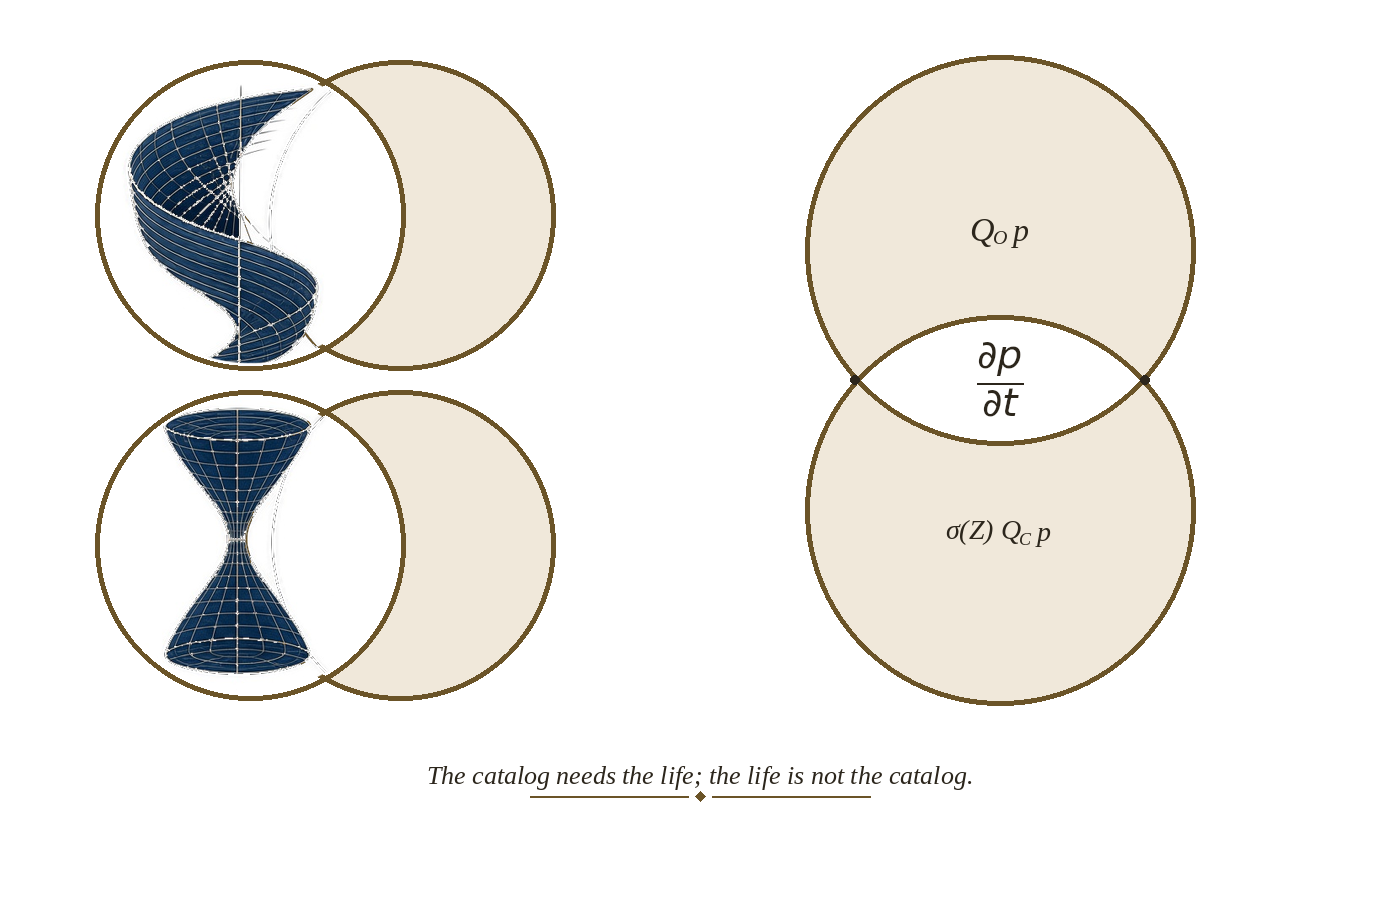
\includegraphics[width=0.88\linewidth]{../fig/formal-full-object.png}
  \caption{Formal full object.
  Life transport \(\QO\) on the helicoid lobe;
  catalog jumps \(\sigma(Z)\,\QC\) on the catenoid lobe;
  the observed motion \(\partial p/\partial t\) only in the lens.
  Surfaces illustrate the split; they are not the configuration manifold.}
  \label{fig:formal}
\end{figure}
